\documentclass[12pt, titlepage]{article}

\usepackage{amsmath, mathtools}

\usepackage[round]{natbib}
\usepackage{amsfonts}
\usepackage{amssymb}
\usepackage{graphicx}
\usepackage{colortbl}
\usepackage{xr}
\usepackage{hyperref}
\usepackage{longtable}
\usepackage{xfrac}
\usepackage{tabularx}
\usepackage{float}
\usepackage{siunitx}
\usepackage{booktabs}
\usepackage{multirow}
\usepackage[section]{placeins}
\usepackage{caption}
\usepackage{fullpage}

\hypersetup{
bookmarks=true,     % show bookmarks bar?
colorlinks=true,       % false: boxed links; true: colored links
linkcolor=red,          % color of internal links (change box color with linkbordercolor)
citecolor=blue,      % color of links to bibliography
filecolor=magenta,  % color of file links
urlcolor=cyan          % color of external links
}

\usepackage{array}

\externaldocument{../../SRS/SRS}

%% Comments

\usepackage{color}

\newif\ifcomments\commentstrue %displays comments
%\newif\ifcomments\commentsfalse %so that comments do not display

\ifcomments
\newcommand{\authornote}[3]{\textcolor{#1}{[#3 ---#2]}}
\newcommand{\todo}[1]{\textcolor{red}{[TODO: #1]}}
\else
\newcommand{\authornote}[3]{}
\newcommand{\todo}[1]{}
\fi

\newcommand{\wss}[1]{\authornote{blue}{SS}{#1}} 
\newcommand{\plt}[1]{\authornote{magenta}{TPLT}{#1}} %For explanation of the template
\newcommand{\an}[1]{\authornote{cyan}{Author}{#1}}

%% Common Parts

\newcommand{\progname}{OCRacle} % PUT YOUR PROGRAM NAME HERE
\newcommand{\authname}{Phillip Tran} % AUTHOR NAMES                  

\usepackage{hyperref}
    \hypersetup{colorlinks=true, linkcolor=blue, citecolor=blue, filecolor=blue,
                urlcolor=blue, unicode=false}
    \urlstyle{same}
                                


\begin{document}

\title{Module Interface Specification for \progname{}}

\author{\authname}

\date{\today}

\maketitle

\pagenumbering{roman}

\section{Revision History}

\begin{tabularx}{\textwidth}{p{3cm}p{2cm}X}
\toprule {\bf Date} & {\bf Version} & {\bf Notes}\\
\midrule
March 13, 2025 & 1.0 & Initial Document Creation\\
\bottomrule
\end{tabularx}

~\newpage

\section{Symbols, Abbreviations and Acronyms}

See SRS Documentation at \url{https://github.com/ptrandev/OCRacle/blob/main/docs/SRS/SRS.pdf}
for symbols, abbreviations and acronyms.

\newpage

\tableofcontents

\newpage

\pagenumbering{arabic}

\section{Introduction}

The following document details the Module Interface Specifications for
\progname{}, an optical character recognition (OCR) program for identifying
Latin alphabet characters.

Complementary documents include the System Requirement Specifications
and Module Guide.  The full documentation and implementation can be
found at \url{https://github.com/ptrandev/OCRacle/}.

\section{Notation}

% \wss{You should describe your notation.  You can use what is below as
%   a starting point.}

The structure of the MIS for modules comes from \citet{HoffmanAndStrooper1995},
with the addition that template modules have been adapted from
\cite{GhezziEtAl2003}.  The mathematical notation comes from Chapter 3 of
\citet{HoffmanAndStrooper1995}.  For instance, the symbol := is used for a
multiple assignment statement and conditional rules follow the form $(c_1
\Rightarrow r_1 | c_2 \Rightarrow r_2 | ... | c_n \Rightarrow r_n )$.

The following table summarizes the primitive data types used by \progname. 

\begin{center}
\renewcommand{\arraystretch}{1.2}
\noindent 
\begin{tabular}{l l p{7.5cm}} 
\toprule 
\textbf{Data Type} & \textbf{Notation} & \textbf{Description}\\ 
\midrule
character & char & a single symbol or digit\\
integer & $\mathbb{Z}$ & a number without a fractional component in (-$\infty$, $\infty$) \\
natural number & $\mathbb{N}$ & a number without a fractional component in [1, $\infty$) \\
real & $\mathbb{R}$ & any number in (-$\infty$, $\infty$)\\
bounded real & $\mathbb{R}_{\text{min} \leq x \leq \text{max}}$ & a real number in the range [$\text{min}$, $\text{max}$]\\
bounded integer & $\mathbb{Z}_{\text{min} \leq x \leq \text{max}}$ & an integer in the range [$\text{min}$, $\text{max}$]\\
boolean & bool & a value that is either true or false\\
\bottomrule
\end{tabular} 
\end{center}

\noindent
The specification of \progname \ uses some derived data types: sequences, strings, and
tuples. Sequences are lists filled with elements of the same data type. Strings
are sequences of characters. Tuples contain a list of values, potentially of
different types. In addition, \progname \ uses functions, which
are defined by the data types of their inputs and outputs. Local functions are
described by giving their type signature followed by their specification.

To describe matrices, the dimensions of the matrix will be described in
superscript (i.e. ${\mathbb{Z}^{w \times w}}$). For all additional notation,
reference Section 1.2 of the SRS Document.
\citep{SRS}.

\section{Module Decomposition}

The following table is taken directly from the Module Guide document for this project.

\begin{table}[h!]
\centering
\begin{tabular}{p{0.3\textwidth} p{0.6\textwidth}}
\toprule
\textbf{Level 1} & \textbf{Level 2}\\
\midrule

{Hardware-Hiding Module} & ~ \\
\midrule

\multirow{8}{0.3\textwidth}{Behaviour-Hiding Module} &
Input Format Module\\
& Model Output Module\\
& Model Training Module\\
& Prediction Model Module\\
& Application Module\\
& Image Preprocessing Module\\
& Accuracy Metrics Module\\
& Data Loading Module\\
\midrule

\multirow{1}{0.3\textwidth}{Software Decision Module}&
Graphical User Interface Module\\
\bottomrule

\end{tabular}
\caption{Module Hierarchy}
\label{TblMH}
\end{table}

\newpage
~\newpage

\section{MIS of Application Module} \label{MApplication}

\subsection{Module}

main

\subsection{Uses}

\begin{itemize}
  \item Input Format Module \ref{MInput}
  \item Model Output Module \ref{MOutput}
  \item Graphical User Interface Module \ref{MGUI}
\end{itemize}

\subsection{Syntax}

\subsubsection{Exported Constants}

N/A

\subsubsection{Exported Access Programs}

\begin{center}
\begin{tabular}{p{2cm} p{4cm} p{4cm} p{2cm}}
\hline
\textbf{Name} & \textbf{In} & \textbf{Out} & \textbf{Exceptions} \\
\hline
main & - & - & - \\
\hline
\end{tabular}
\end{center}

\subsection{Semantics}

\subsubsection{State Variables}

N/A

\subsubsection{Environment Variables}

\begin{itemize}
  \item filePath: string. The path to the input image file from the user.
\end{itemize}

\subsubsection{Assumptions}

The Graphical User Interface module \ref{MGUI} is responsible for handling all
user inputs and displaying outputs The Application module is responsible for
coordinating the interaction between the GUI, Input Format, and Model Output
modules.

\subsubsection{Access Routine Semantics}

\noindent main():
\begin{itemize}
\item transition: The application is started and the user is able to interact
with the GUI to input images and view the model's predictions.
\end{itemize}


\subsubsection{Local Functions}

N/A

\newpage
\section{MIS of Input Format Module} \label{MInput}

\subsection{Module}

input

\subsection{Uses}

\begin{itemize}
  \item Image Preprocessing Module \ref{mPreprocessing}
\end{itemize}

\subsection{Syntax}

\subsubsection{Exported Constants}

N/A

\subsubsection{Exported Access Programs}

\begin{center}
\begin{tabular}{p{2cm} p{2cm} p{3cm} p{6cm}}
\hline
\textbf{Name} & \textbf{In} & \textbf{Out} & \textbf{Exceptions} \\
\hline
input & filePath: string & $\mathbb{Z}^{w \times w}_{0 \le x \le 255}$ & DimensionsError, FormatError, FileNotFound \\
\hline
\end{tabular}
\end{center}

\subsection{Semantics}

\subsubsection{State Variables}

N/A

\subsubsection{Environment Variables}

\begin{itemize}
  \item Image: The input image file to be processed by \progname{}.
\end{itemize}

\subsubsection{Assumptions}

N/A

\subsubsection{Access Routine Semantics}

\noindent input(filePath):
\begin{itemize} 
\item output: imageMatrix := preprocessing(filePath). After ensuring that all
exceptions are handled, call the preprocessing module \ref{mPreprocessing} to
perform the necessary transformations on the input image. \footnote{By splitting
up the file handling concerns with the preprocessing concerns, we are able to
ensure that AC3 and AC5 from the MG \citep{MG} are met. This separation of
concerns allows for better modularity and maintainability of the code. For
instance, if we wanted to be able to support multiple preprocessing methods or
allow input of files other than images.}
\item exceptions:
\begin{itemize}
  \item A DimensionsError exception is thrown if the input image
  exceeds the bounds of the $n_{min}$, $n_{max}$, $m_{min}$, and $m_{max}$
  parameters as specified by Table 4 in the SRS \citep[4.2.6]{SRS}.
  \item A FormatError exception is thrown if the input image is not one of the supported formats
  specified by R1 in the SRS \citep[5.1.1]{SRS}.
  \item A FileNotFound exception is thrown if the input file does not exist.
\end{itemize}
\end{itemize}

\subsubsection{Local Functions}

N/A

\newpage
\section{MIS of Model Output Module} \label{MOutput}

\subsection{Module}

output
\subsection{Uses}

\begin{itemize}
  \item Prediction Model Module \ref{MModel}
\end{itemize}


\subsection{Syntax}

\subsubsection{Exported Constants}

\begin{itemize}
  \item LABELS: ${['A'...'Z']}$
\end{itemize}

\subsubsection{Exported Access Programs}

\begin{center}
\begin{tabular}{p{2cm} p{4cm} p{4cm} p{2cm}}
\hline
\textbf{Name} & \textbf{In} & \textbf{Out} & \textbf{Exceptions} \\
\hline
output & imageMatrix: $\mathbb{Z}^{w \times w}_{0 \le x \le 255}$ & char, $\mathbb{R}_{\text{0} \leq \text{x} \leq \text{1}}^{1 \times L}$ & - \\
\hline
\end{tabular}
\end{center}

\subsection{Semantics}

\subsubsection{State Variables}

N/A

\subsubsection{Environment Variables}

N/A

\subsubsection{Assumptions}

We assume that the imageMatrix input has been processed by the Input Format
Module \ref{MInput} before being passed to the Model Output Module.

\subsubsection{Access Routine Semantics}

\noindent output(imageMatrix):
\begin{itemize}
\item output:
\begin{itemize}
  \item confidenceMatrix := predict(imageMatrix). Call the prediction model
  module \ref{MModel} to generate a confidence matrix for the input image.
  \item prediction := LABELS[argmax(confidenceMatrix)]. Return the character
  representing the highest confidence value in the confidence matrix. When there
  is a tie, the first most confident character is returned.
\end{itemize}
\end{itemize}

\newpage
\section{MIS of Model Training Module} \label{MTraining}

\subsection{Module}

train

\subsection{Uses}

\begin{itemize}
  \item Input Format Module \ref{MInput}
  \item Model Output Module \ref{MOutput}
  \item Prediction Model Module \ref{MModel}
  \item Accuracy Metrics Module \ref{mAccuracy}
\end{itemize}

\subsection{Syntax}

\subsubsection{Exported Constants}

N/A

\subsubsection{Exported Access Programs}

\begin{center}
\begin{tabular}{p{2cm} p{4cm} p{4cm} p{2cm}}
\hline
\textbf{Name} & \textbf{In} & \textbf{Out} & \textbf{Exceptions} \\
\hline
train & - & $\mathbb{R}^{m \times n}$ & - \\
\hline
\end{tabular}
\end{center}

\subsection{Semantics}

\subsubsection{State Variables}

\begin{itemize}
  \item dataset: ($\mathbb{Z}^{w \times w}_{0 \le x \le 255}$, char)[]. The
  dataset of images and their corresponding labels used for training the model.
  \item epochs: $\mathbb{N}$. The number of epochs to train the model.
  \item batchSize: $\mathbb{N}$. The number of images to train on in each batch.
  \item timeStep: $\mathbb{R}$. The time step for the ADAM optimizer.
  \item $\alpha$: $\mathbb{R}$. The rate at which the model learns.
  \item $\epsilon$: $\mathbb{R}$. A small value to prevent division by zero.
  \item $m_{t}$: $\mathbb{R}$. The first moment for the ADAM optimizer.
  \item $v_{t}$: $\mathbb{R}$. The second moment for the ADAM optimizer.
  \item $\beta_1$: $\mathbb{R}$. The $\beta_1$ parameter for the ADAM optimizer.
  \item $\beta_2$: $\mathbb{R}$. The $\beta_2$ parameter for the ADAM optimizer.
  \item $g_{t}$: $\mathbb{R}^{m \times n}$. The gradient of the model. 
  \item $\theta_{t}$: $\mathbb{R}^{m \times n}$. The weights of the model.
\end{itemize}

\subsubsection{Environment Variables}

N/A

\subsubsection{Assumptions}

N/A

\subsubsection{Access Routine Semantics}

\noindent train():
\begin{itemize}
\item transition: The model is trained on the dataset using the hyperparameters
$\alpha$, $\beta_1$, $\beta_2$, $\epsilon$, $m_{t}$, $v_{t}$, $g_{t}$,
$\theta_{t}$, epochs, batchSize, and timeStep. The ADAM optimizer is used to
minimize the cross-entropy loss as specified by TM:ADAM \citep[4.2.2]{SRS} and
IM1 in the SRS \citep[4.2.4]{SRS}. For each step, theta is updated using the
gradient of the model.
\item output: $\theta$. Once the model has been trained and loss has been
minimized, the weights of the model are returned.
\end{itemize}

\subsubsection{Local Functions}

N/A


\newpage
\section{MIS of Prediction Model Module} \label{MModel}

\subsection{Module}

model

\subsection{Uses}

N/A


\subsection{Syntax}

\subsubsection{Exported Constants}

N/A

\subsubsection{Exported Access Programs}

\begin{center}
\begin{tabular}{p{2cm} p{4cm} p{4cm} p{2cm}}
\hline
\textbf{Name} & \textbf{In} & \textbf{Out} & \textbf{Exceptions} \\
\hline
predict & imageMatrix: $\mathbb{Z}^{w \times w}_{0 \le x \le 255}$ & $\mathbb{R}_{\text{0} \leq \text{x} \leq \text{1}}^{1 \times L}$ & - \\
\hline
\end{tabular}
\end{center}

\subsection{Semantics}

\subsubsection{State Variables}

\begin{itemize}
  \item model: $\mathbb{R}^{m \times n}$. The representation of the model's
  weights for the prediction model.
\end{itemize}

\subsubsection{Environment Variables}

N/A

\subsubsection{Assumptions}

We assume that the input image has been preprocessed as specified in the SRS
before being passed to the prediction model.


\subsubsection{Access Routine Semantics}

\noindent predict(imageMatrix):
\begin{itemize}
\item output: confidenceMatrix. Where each element in the confidence matrix
represents the model's confidence in the corresponding character. The model is
used to generate a confidence matrix for the input image using a CNN as
specified by GD3 in the SRS \citep[4.2.3]{SRS}. GD3 provides a high-level
description of the model's architecture, but the implemented model may differ.
\end{itemize}


\subsubsection{Local Functions}

N/A

\newpage
\section{MIS of Image Preprocessing Module} \label{mPreprocessing}

\subsection{Module}

preprocessing

\subsection{Uses}

N/A

\subsection{Syntax}

\subsubsection{Exported Constants}

N/A

\subsubsection{Exported Access Programs}

\begin{center}
\begin{tabular}{p{3cm} p{3cm} p{4cm} p{2cm}}
\hline
\textbf{Name} & \textbf{In} & \textbf{Out} & \textbf{Exceptions} \\
\hline
preprocessing & file : string & $\mathbb{Z}^{w \times w}_{0 \le x \le 255}$ & - \\
\hline
\end{tabular}
\end{center}

\subsection{Semantics}

\subsubsection{State Variables}

N/A

\subsubsection{Environment Variables}

N/A

\subsubsection{Assumptions}

All input data has been validated by the Input Format Module before being
processed by the Image Preprocessing Module.

\subsubsection{Access Routine Semantics}

\noindent preprocessing(file):
\begin{itemize} 
\item output: imageMatrix := normalization(bicubicInterpolation(file)). The
input file has been transformed such that it conforms to the preprocessing
requirements as specified by A3 in the SRS \citep[4.2.1]{SRS}.
\end{itemize}

\subsubsection{Local Functions}

\noindent bicubicInterpolation(imageMatrix):
\begin{itemize}
\item output: Perform bicubic interpolation such that the imageMatrix is
transformed to a ${w times w}$ matrix. as specified by TM:BI in the SRS \citep[4.2.2]{SRS}.
\end{itemize}
\noindent normalization(imageMatrix):
\begin{itemize}
\item output: Perform normalization such that the image is turned into a
greyscale image with pixel values in the range [0, 255]. as specified by TM:N in
the SRS \citep[4.2.2]{SRS}.
\end{itemize}

\newpage
\section{MIS of Accuracy Metrics Module} \label{mAccuracy}

\subsection{Module}

performance

\subsection{Uses}

N/A


\subsection{Syntax}

\subsubsection{Exported Constants}

N/A

\subsubsection{Exported Access Programs}

\begin{center}
\begin{tabular}{p{4cm} p{4cm} p{4cm} p{2cm}}
\hline
\textbf{Name} & \textbf{In} & \textbf{Out} & \textbf{Exceptions} \\
\hline
crossEntropyLoss & prediction: $\mathbb{R}_{\text{0} \leq \text{x} \leq \text{1}}^{1 \times L}$, target: $\mathbb{R}_{\text{0} \leq \text{x} \leq \text{1}}^{1 \times L}$ & loss: $\mathbb{R_{\text{0} \leq \text{x} \leq \text{1}}}$ & DimensionsError \\
confusionMatrix & prediction: $\mathbb{R}_{\text{0} \leq \text{x} \leq \text{1}}^{1 \times L}$, target: $\mathbb{R}_{\text{0} \leq \text{x} \leq \text{1}}^{1 \times L}$ & confusionMatrix: $\mathbb{R_{\text{0} \leq \text{x} \leq \text{1}}}^{26 \times 26}$ & DimensionsError \\
\hline
\end{tabular}
\end{center}

\subsection{Semantics}

\subsubsection{State Variables}

N/A

\subsubsection{Environment Variables}

N/A

\subsubsection{Assumptions}

N/A

\subsubsection{Access Routine Semantics}

\noindent crossEntropyLoss(prediction, target):
\begin{itemize}
\item output: loss := $- \sum_{i=1}^{n} target_i \log(prediction_i)$. The cross
entropy loss is calculated for the model's predictions and the target values
as specified by TM:CELF in the SRS \cite[4.2.2]{SRS}.
\item exceptions:
\begin{itemize}
  \item A DimensionsError exception is thrown if the dimensions of the prediction
  and target matrices do not match.
\end{itemize}
\end{itemize}

\noindent confusionMatrix(prediction, target):
\begin{itemize}
\item output: confusionMatrix := $\text{confusionMatrix}_{i,j} = \sum_{k=1}^{n} \text{target}_{k,i} \times \text{prediction}_{k,j}$. A confusion matrix is generated for the
model's predictions and the target values to fulfill NFR1 in the SRS
\cite[5.2]{SRS}.
\item exceptions:
\begin{itemize}
  \item A DimensionsError exception is thrown if the dimensions of the prediction
  and target matrices do not match.
\end{itemize}
\end{itemize}

\subsubsection{Local Functions}

N/A

\newpage
\section{MIS of Data Loading Module} \label{MDataLoading}

\subsection{Module}

data
\subsection{Uses}

N/A

\subsection{Syntax}

\subsubsection{Exported Constants}

N/A

\subsubsection{Exported Access Programs}


\begin{center}
\begin{tabular}{p{5cm} p{2cm} p{4cm} p{2cm}}
\hline
\textbf{Name} & \textbf{In} & \textbf{Out} & \textbf{Exceptions} \\
\hline
extractTestSamples & - & ${\mathbb{R}^{w \times w}_{0 \ge x \ge 1}[]}$, ${\mathbb{Z}[]}$ & - \\
extractTrainingSamples & - & ${\mathbb{R}^{w \times w}_{0 \ge x \ge 1}[]}$, ${\mathbb{Z}[]}$ & - \\
\hline
\end{tabular}
\end{center}

\subsection{Semantics}

\subsubsection{State Variables}

N/A

\subsubsection{Environment Variables}

N/A

\subsubsection{Assumptions}

N/A

\subsubsection{Access Routine Semantics}

\noindent extractTestSamples():
\begin{itemize}
\item output: (images, labels) := processSamples(testImages, testLabels). A
tuple containing the test images and their corresponding labels. The test
samples are extracted from the EMNIST letters dataset.
\end{itemize}

\noindent extractTrainingSamples():
\begin{itemize}
\item output: (images, labels) := processSamples(trainingImages, trainingLabels).
A tuple containing the training images and their corresponding labels. The
training samples are extracted from the EMNIST letters dataset.
\end{itemize}

\subsubsection{Local Functions}

\noindent processSamples():
\begin{itemize}
\item output: (images, labels). The images are normalized to have a pixel range
between 0 and 1 inclusive, as specified by the SRS document \citep{SRS}. The
labels are scaled to start at 0 instead of 1 to align with the model
architecture's output as specified by the SRS document \citep{SRS}.
\end{itemize}


\newpage
\section{MIS of Graphical User Interface Module} \label{MGUI}

\subsection{Module}

gui
\subsection{Uses}

\begin{itemize}
  \item Hardware-Hiding Module
\end{itemize}

\subsection{Syntax}

\subsubsection{Exported Constants}

N/A

\subsubsection{Exported Access Programs}


View the Appendix \ref{Appendix} for more information the full range of
interactions that the Graphical User Interface Module can have with the user.

\begin{center}
\begin{tabular}{p{4cm} p{4cm} p{4cm} p{2cm}}
\hline
\textbf{Name} & \textbf{In} & \textbf{Out} & \textbf{Exceptions} \\
\hline
displayOutput & - & - & - \\
acceptInput & - & - & - \\
\hline
\end{tabular}
\end{center}

\subsection{Semantics}

\subsubsection{State Variables}

N/A

\subsubsection{Environment Variables}

\begin{itemize}
  \item displayWindow: (dimensions: $\mathbb{Z}_+ \times \mathbb{Z}_+$)
  \item keyboard: (keypress: char)
  \item mouse: (location: $\mathbb{Z}_+ \times \mathbb{Z}_+$, click: bool)
\end{itemize}

\subsubsection{Assumptions}

This behavior will be significantly abstracted by the use of Python Notebook,
which will handle all UI elements and interactions with the user. As a result,
the GUI modules does not need to have any pre-defined state variables or access
routines.

\subsubsection{Access Routine Semantics}

\noindent displayOutput():
\begin{itemize}
\item transition: The output of the model is displayed to the user in the GUI.
\end{itemize}

\begin{figure}
\centering
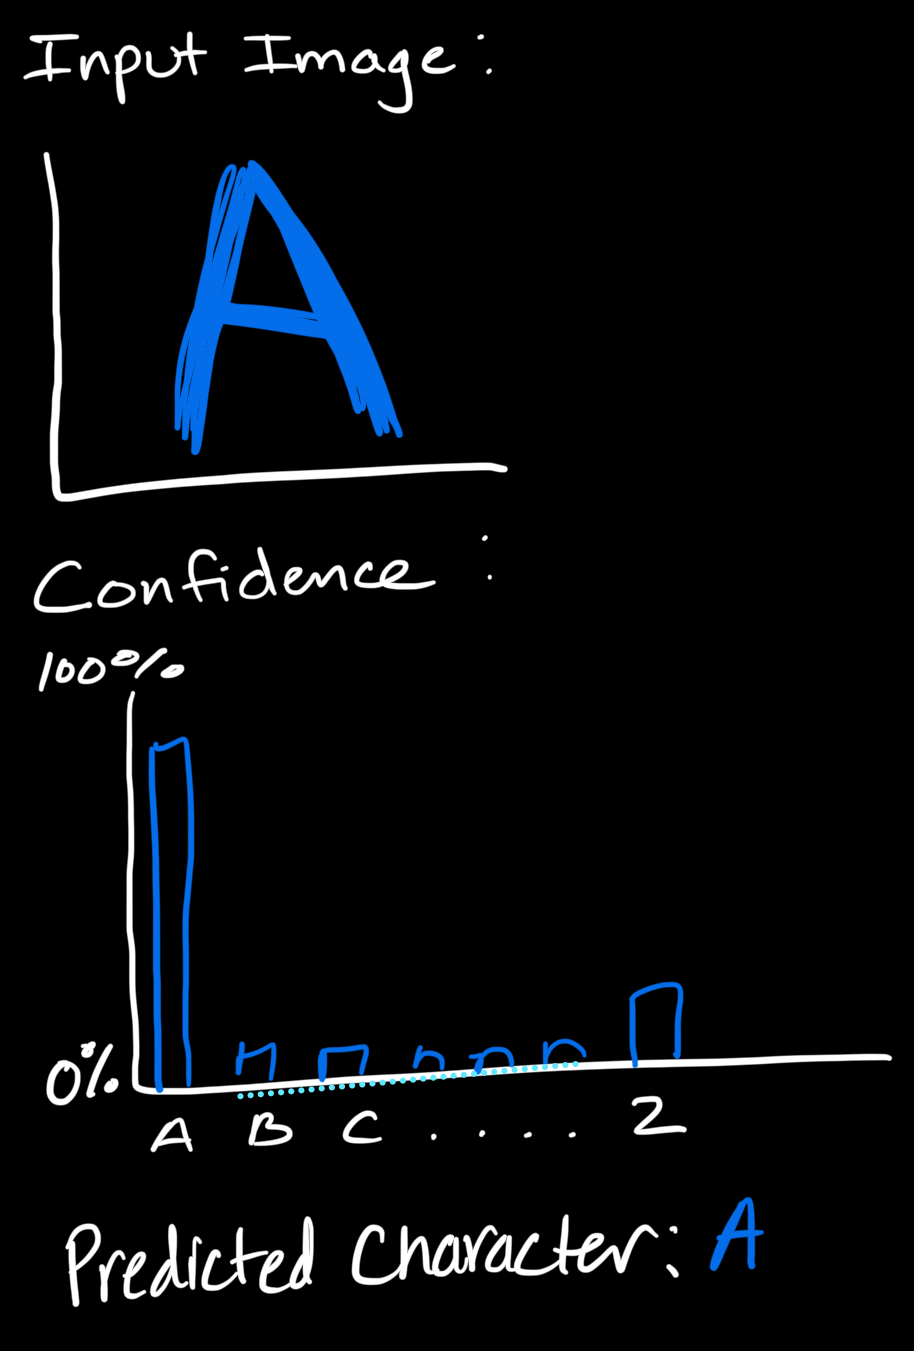
\includegraphics[width=0.5\textwidth]{displayOutput.jpeg}
\caption{Example of the displayOutput() function. It will display the
  model's prediction and the confidence matrix to the user in a graphical
  format.}
\label{fig:displayOutput}
\end{figure}

\noindent acceptInput():
\begin{itemize}
\item transition: The user is able to input images to the model in the GUI.
\end{itemize}

\begin{figure}
  \centering
  
\includegraphics[width=1\textwidth]{acceptInput.jpeg}
  \caption{Example of the acceptInput() function. It allows users to input a
  file path and run the model on the input image.}
  \label{fig:acceptInput}
  \end{figure}

\subsubsection{Local Functions}

N/A

\newpage

\bibliographystyle {plainnat}
\bibliography {../../../refs/References}

\newpage

\section{Appendix} \label{Appendix}

\begin{itemize}
  \item The Python Notebook documentation can be found at
  \url{https://jupyter-notebook.readthedocs.io/en/latest/user-documentation.html}.
  This informs the full range of interactions that the Graphical User Interface
  Module \ref{MGUI} can have with the user.
  \item Generative AI Acknowledgement: ChatGPT-4o was used to generate valid
  LaTeX for mathematical expressions in this document.
\end{itemize}

\newpage{}

\end{document}